
\chapter{Methodology}

One of the main aims of the thesis was to develop a pipeline for statistical analysis of available protein structure annotations (hereinafter referred to as features), and to prepare this pipeline for adding user-defined custom features.

The pipeline is able to do all steps needed for the task, from downloading the structures from PDB, to computing the statistical significance of individual features. Moreover, there are two scripts that further extend the analysis pipeline and can be used to train and evaluate P2Rank models with new features. The only needed input is a dataset file with listed proteins.

The pipeline is implemented in Python, making use of several Python packages, such as BioPython \cite{biopython}, NumPy \cite{numpy} or Matplotlib \cite{maplotlib}. BioPython is an open-source collection of Python tools for computational biology and it was very useful for this work. The main script \texttt{analysis\_pipeline.py} defines the user API, parses and checks arguments, takes care of logging and runs individual parts of the pipeline. See \url{ https://github.com/katebrich/Master-thesis/tree/dev/Scripts} TODO for more details about options, requirements, input, output and examples of usage.

The structure of the pipeline is depicted in Diagram~\ref{fig:diagram}. The details about individual parts are described in this chapter.

\begin{figure}[!htbp]\centering
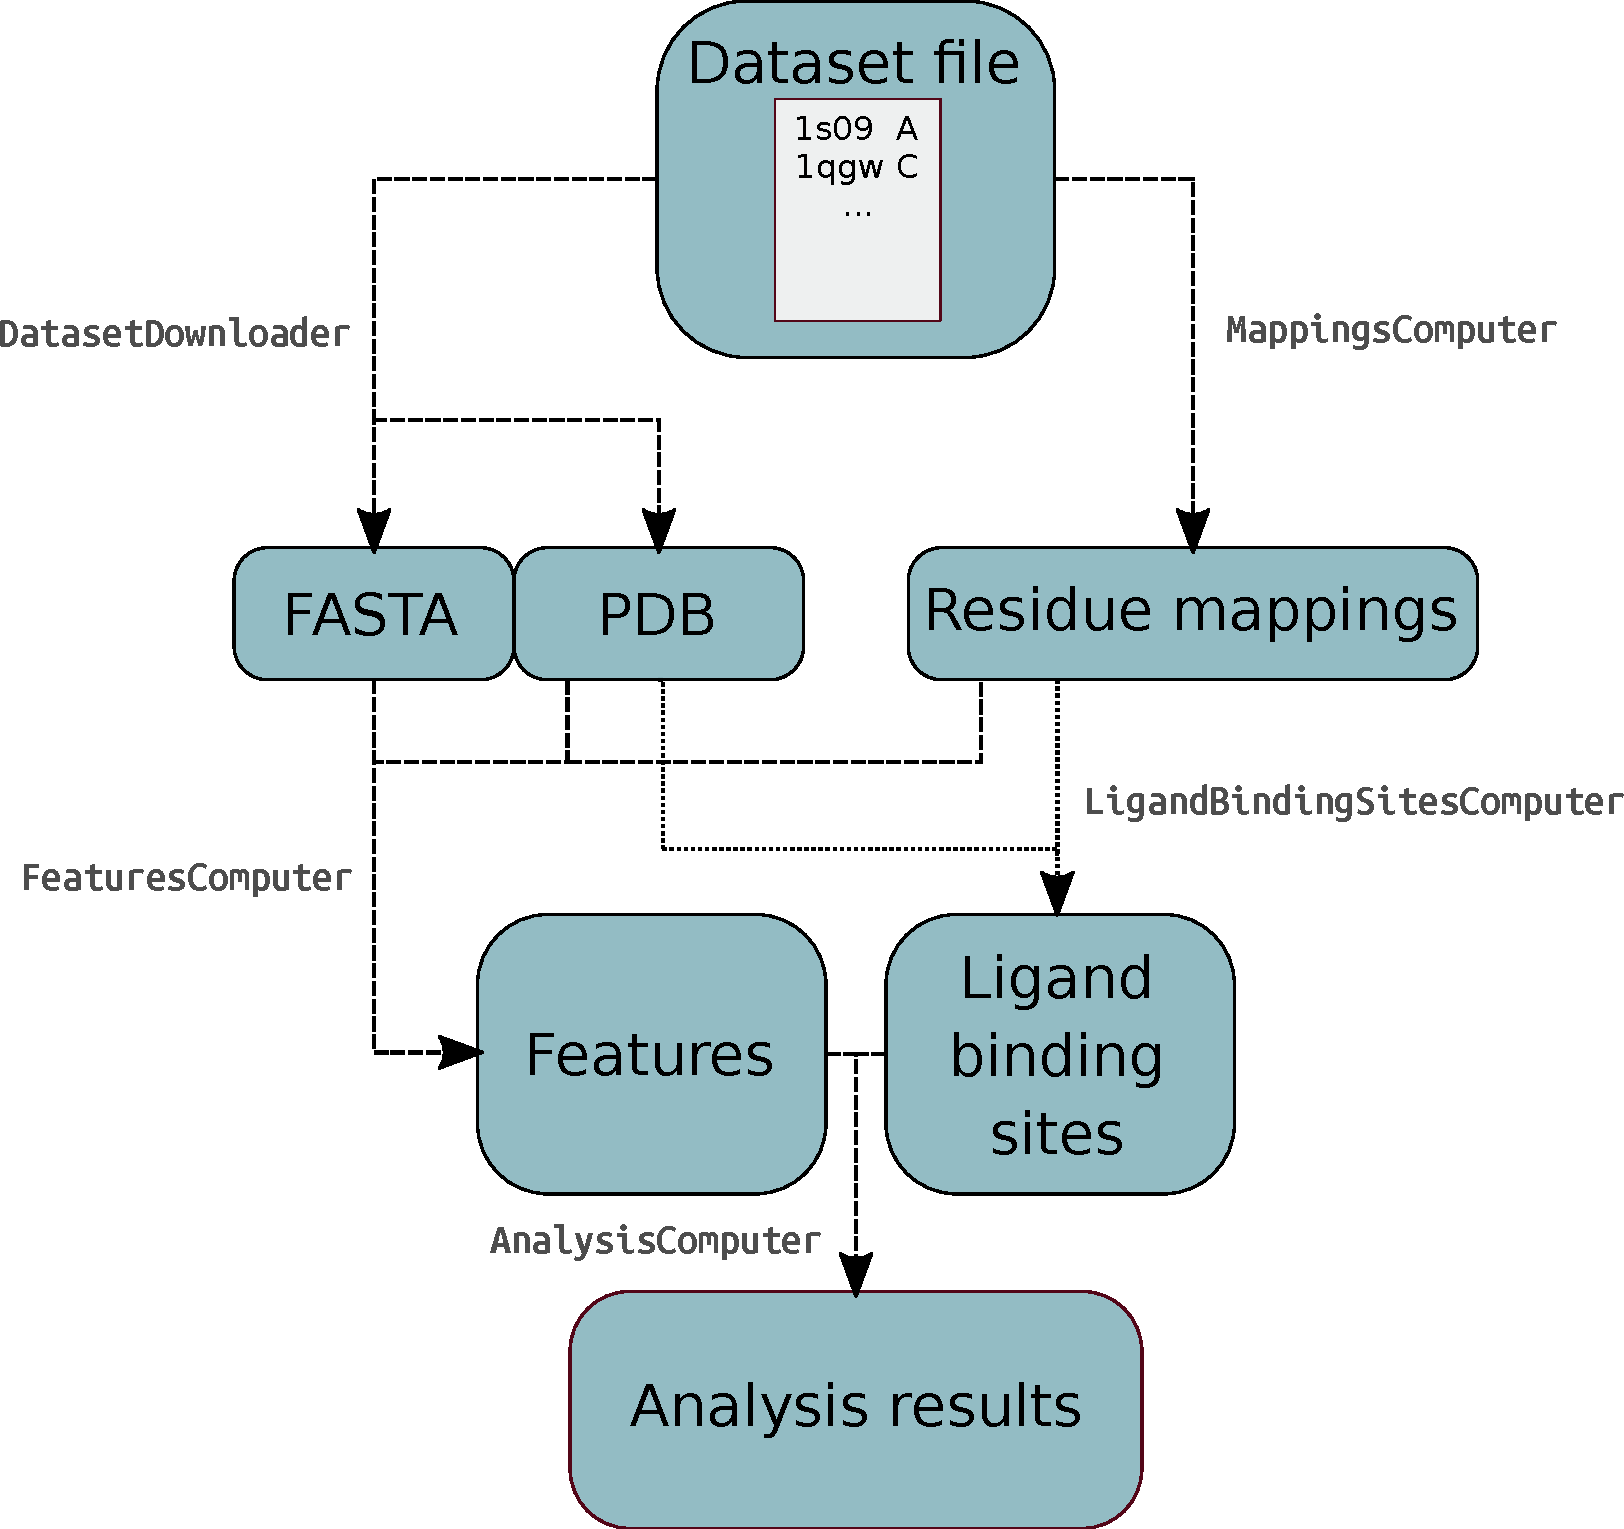
\includegraphics[width=120mm]{../img/pipelineDiagram.pdf}
\caption{Diagram of the pipeline structure.}
\label{fig:diagram}
\end{figure}


TODO verze programu a databazi? Kam to dat?
TODO options, parameters - tasks, threads, output\_dir, dataset
TODO default values

\section{Dataset file}
TODO co je REST API

\section{Data download}

\section{Residue mappings}
- zminit chybu s mapovanim segmentu, insertion codes, proc nesly SIFTS

\section{Ligand binding sites labelling}
- options - lbs\_distance\_threshold
- problemy s HETATM
- SASA + cutoff

\section{Features}

....TODO
- options - features, config\_path

\subsection{UniProtKB}

The UniProt Knowledgebase (UniProtKB) is a large database of well-annotated protein sequence data. It tries to achieve the minimal redundancy and it provides detailed, accurate and consistent annotations of the sequences \cite{uniprot}.

Sequence annotations (called `features') are available for every UniProtKB entry. They describe interesting sites and regions on the protein sequence and every feature has an associated description with more information, such as available evidence, source or related publications. The features are arranged in a well-organized manner on the website, in so called `Features viewer' with many overlapping tracks for different features. Nonetheless, for the purpose of this work, the best way to obtain the features was via the Proteins REST API \cite{proteins_api}. It provides the interface to  access the sequence annotation data as well as mapped variation data programmatically. The API is available at (\url{http://www.ebi.ac.uk/proteins/api/doc}) \cite{TODO}.

Features are classified into eight categories which are further subdivided into types. For example, the category `STRUCTURAL' comprises the types `HELIX', `TURN' and `STRAND'.

The types and categories that were chosen as potentially relevant for ligand binding sites prediction are described below.


\subsubsection{PTM}
Post-translational modifications are covalent chemical modifications of polypeptide chains after translation, usually modifying the functional group of the standard amino acids, or introducing a new group. They extend the set of the 20 standard amino acids and they can be important for the function of many proteins,as they can alter the interactions with other proteins, localization, activity, signal transduction, cell-cell interactions and other properties. Their enrichment in binding sites is very interesting to examine.

Three UniProtKB feature types were analysed: lipidation, glycosylation and type `MOD\_RES' which comprises phosphorylation, methylation, acetylation, amidation, formation of pyrrolidone carboxylic acid, isomerization, hydroxylation, sulfation, flavin-binding, cysteine oxidation and nitrosylation. Only experimentally determined modification sites are annotated, and they are further propagated to related orthologs when specific criteria are met \cite{mod_res}.

Since lipidaton and glycosylation data were very sparse (e.g. there were only 15 lipidation sites in the whole holo4k dataset composed of 3973 proteins), the fourth feature called `PTM' including all three types was added to the analysis.

\subsubsection{Disulfide bonds}
Another type of post-translational modifications are disulfide bonds formed between two cysteine residues. Both intrachain and interchain bonds are annotated by \mbox{UniProtKB}. The disulfide bonds may be either experimentally determined or predicted \cite{disulfid}.

\subsubsection{Non-standard residues}
Describes the occurence of non-standard amino acids (selenocysteine and pyrrolysine). There must be experimental evidence for this occurence; however, it can be propagated to close homologs \cite{non_std}.

\subsubsection{Secondary structure}
This feature category annotates three types of secondary structures: helices, beta sheets and hydrogen-bonded turns. Residues not belonging to any of the classes are in a random-coil structure. The `helix' class comprises alpha-helices, pi-helices and 3\textsubscript{10} helices.

The secondary structure assignment is made by DSSP algorithm \cite{dssp} based on the coordinate data sets extracted from the Protein Data Bank (PDB). They are neither predicted computationally, nor propagated to related species \cite{sec_str}.

\subsubsection{Natural variant}
This feature includes naturally occuring polymorphisms, variations between strains or RNA editing events \cite{natural_variant}.

\subsubsection{Variation}
\textit{Variation service} is a utility that can retrieve variation data from UniProtKB. The variants are either extracted from the scientific literature and manually reviewed, or mapped from large scale studies, such as 1000 Genomes \cite{1000genomes}, COSMIC \cite{cosmic}, ClinVar \cite{clinvar} or ExAC \cite{exac}. The Proteins REST API provides various options for variants retrieval, such as to filter by the consequence type, associated disease name, cross reference database type (e.g. ClinVar) or by the source type \cite{proteins_api}.


\subsubsection{Compositional bias}
The regions of compositional bias are parts of the polypeptide chain where some of the amino acids are over-represented, not following the standard frequencies. The regions can be enriched in one or more different amino acids \cite{https://www.uniprot.org/help/compbias}.



\subsection{PDBe-KB}
PDBe-KB (Protein Data Bank in Europe - Knowledge Base) is managed by the PDBe team at the European Bioinformatics Institute. It is a collaborative resource that aims to bring together the annotations from various sources and to show the macromolecular structures in broader biological context. 

One drawback of PDB is that every page represents only one entry that is based on a single experiment. There may be several PDB entries for the full-length protein, each covering only a segment of it. Nevertheless, the entries for the same protein are not interconnected. PDBe-KB has developed the \textit{aggregated views of proteins}, displaying an overview of all the data related to the full-length protein defined by the UniProtKB accession.

The structures from the PDB are extensively used by scientific software and other resources. There exist many valuable annotations, such as ligand binding sites, post-translational modification sites, molecular channels or effects of mutations, that are created outside of the PDB. The problem is that the data is fragmented and therefore it would require immense effort of a researcher to collect and make use of all available data for a structure of interest.

The aggregated views of proteins integrates the annotations from \textit{PDBe-KB partners}, collaborating scientific software developers. It facilitates the retrieval of these annotations with a uniform data access mechanism (via FTP or REST API). The project is called `FunPDBe'. A common data exchange scheme was defined to facilitate the transfer of data. \cite{pdbekb}

The use of PDBe-KB was difficult because of the lack of documentation and a few bugs that were encountered during this work (some of them corrected by now after pointing them out). However, it is understandable since it was launched only two years ago and the constant improvements are done since then.

\subsubsection{Conservation}
PDBe-KB provides pre-calculated residue-level conservation scores, obtained by a pipeline using HMMER and Skylign web servers that was described by Jakubec et al. \cite{3dpatch}.

The values of the score are integers ranging from 0 to 9, with 9 being the most conserved. Since scores higher than 4 were very sparse and the feature would not meet the assumptions of the Chi-squared test, the scores 4 and higher were merged into one category (4). This does not deteriorate the prediction nor the hypothesis test, as vast majority (over 95\%) of non-binding residues were scored 1 and lower.

\subsubsection{DynaMine}
DynaMine was developed by the Bio2Byte group \cite{bio2byte} and it is one of the PDBe-KB partner resources. It provides the annotations of the backbone dynamics predicted only from the FASTA sequence. DynaMine predicts backbone flexibility at the residue-level, using a linear regression model trained on a large dataset of curated NMR chemical shifts extracted from the Biological Magnetic Resonance Data Bank \cite{bmrb}. The predictor estimates the value of the `order parameter' (S\textsuperscript{2}) which is related to the rotational freedom of the N-H bond vector of the backbone. The values range from 0 (highly dynamic) to 1 (complete order) \cite{dynamine}.

\subsubsection{EFoldMine}
EFoldMine tool comes from the same group as DynaMine. It is a predictor of the early folding regions of proteins. It makes predictions at the residue-level derived only from the FASTA sequence. Internally it uses dynamics predictions and secondary structure propensities as features and the linear regression model is trained on data from NMR pulsed labelling experiments. Unfortunatelly, the early stages of protein folding are not understood very well so far and experimental data is very difficult to obtain. The predictor was trained on the dataset of only 30 proteins and its performance is quite poor \cite{efoldmine}.

\subsubsection{Depth}
Depth is a webserver that can measure residue burial within the protein. It is able to find small cavities in proteins and could be used as a ligand-binding sites predictor as such. The residue depth values are computed from the input PDB file.

The algorithm places input 3D structure in the box of model water, each residue with at least two hydration shells around itself. The water molecules in cavities are removed: the algorithm removes the water molecule if there are less than a given number of water molecules in its spherical volume of given size. The minimum number of neighbouring molecules and the spherical volume can be defined by the user. The removal is iterated until there are no more cavity waters. Residue depth is then computed as the distance to the closest water molecule \cite{depth}.


\subsection{PDB}

\subsubsection{B factor}

\subsubsection{Half sphere exposure}

\subsubsection{Exposure CN}

\subsubsection{Phi and psi angles}

\subsubsection{Cis peptide}




\subsection{FASTA}



\subsection{Other resources}

\subsubsection{MobiDB}

\subsubsection{Conservation}


\subsection{Custom features}




\section{Statistical analysis}

TODO P-value
TODO power of test

TODO implementace testu v Pythonu

To find properties mapped on the protein primary structure which are possibly important for prediction of protein-ligand binding sites, statistical analysis will have the crucial role. It is a great way to explore the big amounts of accessible data and it can potentially help to discover underlying patterns and draw inferences from the data.

This chapter describes the method that was used to analyse the \textit{statistical significance} of the properties and to distinguish the ones that stand out in the known protein-ligand binding sites.



Hypothesis testing is a method of statistical inference. Its goal is to infer properties of a \textit{statistical population}, i.e. a set of similar items or events. In this work, two populations will be compared: we take values of a property for all the amino acids across all the proteins in the dataset and then compare the ones in binding sites and outside of binding sites.

A dataset usually contains a subset sampled from a larger population, rather than the whole population. This subset is called a \textit{statistical sample}. It should represent the population well and be unbiased.

A \textit{hypothesis} makes a statement about an unknown population parameter. In a hypothesis testing problem, an experimenter states two complementary hypotheses: the \textit{null hypothesis} and the \textit{alternative hypothesis}, denoted by $H_{0}$ and $H_{1}$, respectively. The null hypothesis comprises a subset of possible parameters and the alternative hypothesis comprises the supplement, so that all the possible parameters are covered.

In a hypothesis testing problem, an experimenter should come to one of the conclusions: to either accept $H_{0}$, or to reject $H_{0}$ and accept $H_{1}$.

To decide which one of two complementary hypotheses is true, an experimenter employes a suitable \textit{hypothesis test}. A hypothesis test is a rule that specifies for which sample values the $H_{0}$ is accepted as true and for which sample values it is rejected, and therefore $H_{1}$ is accepted as true. A hypothesis test is usually specified in terms of a test statistic (i.e. a function of the sample) \cite{casella}.

As one may expect, the tests are not error-proof and a mistake can be made in the decision of whether to accept or reject the null hypothesis. There are two types of errors in hypothesis testing, commonly known as \textit{Type I error} and \textit{Type II error}. The test has made a Type I error if it incorrectly rejects a true null hypothesis. If, on the other hand, a null hypothesis is accepted and it is not true, a Type II error has been made. Both situations are depicted in the Table~\ref{tab:hypothesis_testing_errors}. The ideal test would have both error probabilities equal to zero. Nevertheless, in most cases it is not possible to make both error probabilities arbitrarily small for a fixed sample size \cite{casella}.

\begin{table}[!htbp]
\centering
\renewcommand{\arraystretch}{2.5}
\begin{tabular}{l|l|c|c|}
\multicolumn{2}{c}{}&\multicolumn{2}{c}{\begin{large}Prediction \end{large}}\\
\cline{3-4}
\multicolumn{2}{c|}{}&Accept $H_{0}$&Reject $H_{0}$\\
\cline{2-4}
\multirow{2}{*}{\begin{large}Truth\end{large}}& \textbf{$H_{0}$} & \shortstack{Correct\\(true positive)} & \shortstack{\textbf{Type I error}\\(false positive)}\\
\cline{2-4}
& \textbf{$H_{1}$} & \shortstack{\textbf{Type II error}\\(false negative)} & \shortstack{Correct\\(true negative)} \\
\cline{2-4}
\end{tabular}
\caption{Type I and II Error in hypothesis testing.}\label{tab:hypothesis_testing_errors}
\end{table}

To control statistical significance of the result, a study defines a threshold called \textit{significance level}, a constant denoted by $\alpha$. It represents the probability  of making a Type I error, in other words, the probability that the study rejects the null hypothesis when it is true.

One way to report the result of the test would be simply to tell whether the null hypothesis was accepted or rejected at the given significance level. However, most researchers choose to report a certain kind of test statistic (function of a sample $X$), the so-called \textit{p-value}.
Smaller values of $p(X)$ give stronger evidence for rejecting the null hypothesis. The null hypothesis is rejected when $p(X) \leq \alpha$. Hence, we are able to determine the smallest significance level at which the hypothesis would be accepted/rejected. P-value gives an idea of how strongly the data contradict the null hypothesis; furthermore, it allows other researchers to make a decision according to the significance level of their choice \cite{sham_purcell, casella, lehmann}.

It is suggested that the significance level for a study is set prior to any data collection \cite{neynman_pearson}. The typical choices in practice are $\alpha =$ 0.01, 0.05 or 0.10 \cite{casella}. One should be aware that by fixing the significance level of the test, the experimenter is controlling only the Type I error probabilities. The probability of the Type II error is subject to factors such as the accuracy and completeness of the data and most importantly, the true effect size \cite{sham_purcell}.

Let's suppose an experimenter has a research hypothesis that he or she hopes to prove, but does not want to risk accepting it without convincing data support. In this case, the test should be set up in such a way that the research hypothesis corresponds to the alternative hypothesis, not the null hypothesis. By specifying a small significance level $\alpha$, the experimenter thus controls the probability of the Type I error. In other words, the probability of accepting the research hypothesis when in is not true would be $\alpha$ at most \cite{casella}.



\subsection{Welch's test}

Welch's unequal variances t-test, or Welch's test in short, is a two-sample hypothesis test used to decide whether two populations have different central tendencies (means or medians). The decision is made based on the samples from the two populations. It is a more robust alteration of the widely used Student's t-test \cite{welch}.

Both Student's and Welch's t-test assume that the two examined populations follow a normal distribution \cite{welch}. Nevertheless, when testing for the equality of means of ``large enough samples'', the normality assumption can be violated thanks to the large sample theory and the Central Limit Theorem \cite{lehmann}. It has been shown in previous studies that for large samples, the statistical significance level is protected not only for normally distributed data, but also for many non-normal distributions; moreover, in case of Welch's test, this is true even for unequal variances \cite{zimmerman_zumbo_1993, zumbo_coulombe_1997, lumley}. According to  Lehmann and Romano \cite{lehmann}, the Type II error is also relatively insensitive to non-normality. Many articles and textbooks mention that when the sample sizes are small, nonparametric tests (i.e. tests that do not assume a specific distribution) such as the Mann-Whitney test \cite{mann} should be considered as an alternative to t-tests.
However, t-tests become superior when sample sizes increase \cite{zimmerman1998, lumley}. The simulations made by Lumley \textit{et al.} \cite{lumley} show that ``sufficiently large sample size'' means under 100 in most cases. Even for extremely non-normal data, the sufficient size is at most 500. This suggests that the choice of Welch's test is legitimate for this work.

The problem of the Student's t-test is that it performs badly when the variances of the two compared populations are unequal. Both Type I and Type II errors are negatively affected by violation of the equal variances assumption. The unequal variances can be less problematic if sample sizes are similar, but in practice, that is not always the case \cite{ruxton}.

Unlike Student's t-test, Welch's test does not assume equal variances of the populations. It performs well when the samples have unequal variances; furthermore, it can be used even when the samples have unequal sizes \cite{derrick}.

Some researchers tend to pre-test for variance equality by a preliminary test of variances (such as Levene's \cite{levene}, Bartlett's \cite{bartlett} or Brown-Forsythe test \cite{brown}) and then choose whether to use Student's or Welch's t-test. However, although this approach persists in some textbooks and software packages, it is not recommended by statisticians. As a preliminary test itself is subject to Type I and II errors, this two-stage procedure would not protect the significance level and could lead to incorrect decisions. One should be aware of the fact that even if the test suggested that the samples variances are nearly equal, it would not mean that the whole population variances could not differ to a larger extent \cite{zimmerman}. Some researchers may try to make the significance level of a preliminary test more strict, so that they could be more confident about the choice of the subsequent test; however, as the significance level decreases, the performance of the compound test paradoxically gets worse. According to Zimmerman \cite{zimmerman}, ``a higher Type I error rate of the preliminary test actually improves the performance of the compound test''. This suggests that using the preliminary test is not correct in principle.

Welch's test should be used whenever the researcher is not sure that the variances are truly equal. Ruxton \cite{ruxton} even suggests the routine use of Welch's test. When the sample sizes and variances are equal, both tests perform similarly. When dealing with unequal variances and unequal sample sizes, Welch's test is more robust than Student's t-test and the Type I error rate does not deviate far from the nominal value \cite{derrick}. Hence, Welch's test can be applied without any significant disadvantages to Student's t-test.

For all the reasons stated above, Welch's test seems to be the best choice for the purpose of this study. It has the best combination of performance and ease of use, the calculation is straightforward and it is available in commonly used statistics packages.

\subsection{Chi-squared test of independence}

A different kind of tests will be needed for the analysis of categorical features. An example of a categorical feature is XXX. Moreover, quantitative features can be grouped into categories and analysed in the same way as categorical features. In this section, two widely-used tests of such kind will be presented and discussed.

Both Fisher's exact test and Chi-squared test of independence are well-known hypothesis tests used for the analysis of data in contigency tables. A \textit{contigency table} is a table displayed in a form of a matrix where cells represent a frequency distribution of samples in the categories. An example of a contingency table can be seen in Table~\ref{tab:contingency_table_example}. The sums of frequencies in rows and columns are called \textit{marginal totals}.

\begin{table}[!htbp]
\centering
\renewcommand{\arraystretch}{1.5}
\newcolumntype{s}{>{\columncolor{lightgray}} p{3cm}}
 \begin{tabular}{|c|c|c||c|} 
 \hline
  & PTM & Without PTM & Total \\ [0.5ex] 
 \hline
 Binding sites & XX & XX & XX \\ 
 \hline
 Non-binding sites & XX & XX & XX \\
 \hline\hline
 Total & XX & XX & XX \\
 \hline
\end{tabular}
\caption{A $2\times 2$ contingency table. TODO real data}\label{tab:contingency_table_example}
\end{table}

The null hypothesis assumes independence of the groups; in our case, the assumption is that there is no difference in the proportions of the analysed feature between binding sites and non-binding sites.

Fisher's exact test belongs to a class of so-called \textit{exact tests}; it means that the p-value is calculated accurately, not approximately, as is the case of many tests including Welch's test and Chi-squared test. Fisher's test is mostly used for $2\times 2$ contigency tables, although the principle of the computation can be extended to a general $m\times n$ table \cite{Mehta}. The principle of the test lies in computing the probability of obtaining a table that is more or equally extreme in the departure from the null hypothesis than the analysed table and has identical marginal totals \cite{bland}.

Chi-squared ($\chi^{2}$) test if independence is able to decide whether the difference between the observed frequencies and the ``expected frequencies'' is statistically significant. The expected frequencies are computed for every cell as 
$\dfrac{row\: total\times column\:total}{grand\:total}$.
It can be imagined as the average frequencies we would get in the long run with the same marginal totals, assuming the null hypothesis is true (i.e. there is no association between groups). The result of the test tells how likely are we to observe given data under the assumption of the true null hypothesis \cite{bland}. TODO vysvetlit chi-sq rozdeleni a to jak se pocita ta testova statistika

The biggest difference between the two mentioned tests is that the chi-squared test is based on a aproximation approach; therefore, it needs a ``large enough'' sample. TODO FISHERUV TEST OBECNE NA MENSI VZORKY, .... W. G. Cochran (1954) \cite{cochran} proposed a set of recommendations about the minimum expectations to be used in $\chi^{2}$ tests and about the choice between Fisher's test and $\chi^{2}$ test:


These recommendations are presented in several textbooks and articles as a rule of thumb \cite{} and recommended to be used in practice.


TODO: for small, sparse, or unbalanced data, the exact and asymptotic p-values can be quite different and may lead to opposite conclusions concerning the hypothesis of interest. (wikipedia)


\section{P2Rank models training and evaluation}




